
\section{Friday 0601}

\subsection{T1: Modelling NL, programs, and their intersection}

\paragraph{Speakers} Professors Graham Neubig and Miltos Allamanis for sharing the slides.

\subsubsection{Programming language vs natural language}
- a lot of similarities between programming languages and domain-specific languages \\
- data sources available. e.g: Stack Overflow\\
- Categories of data: intent, written intent, code snippets, doc strings, comments, diff messages\\


\subsubsection{Methods for mapping code to natural language}
\begin{itemize}
	\item Translation: (natural language description). Methods: machine translation, CNN + attentions, etc.
	\item Code summarization. e.g: Iyer et al "summarizing source code using a neural attention model". e.g: predict method names
	\item Convolutional neural attention models with attention mechanisms (which decide whether copy or summarize, similar to pointer-generator network)
	\item Incorporating the execution results to evaluate quality of generated programs
	\item Programming by demonstration...?
	\item Semantic parsing from Q-A pairs. Weak supervision is easier to create (e.g: for generating SQL. Zhong+17, Clarke+10)
\end{itemize}

\subsubsection{Program generation: map from language to code}
\begin{itemize}
	\item Machine translation, but with clear destination syntax rules
	\item Historical methods: rule-based transformations, grammar-based models, neural models. Following talks about neural approaches.
	\item How to take advantages of features of code? e.g: copy variable names. (word-level or character-level, or tree-level (Dong+16)) e.g: Top-down generation of CFG rules
	\item Also possible to generate codes from coarse-to-fine level (Dong+18). First predict the sketches, and then codes
	\item Code synthesis with natural language guidance (Polosukhin+18)
	\item Reconstruction loss: supervision without execution (Yin+18). Can use VAE formulation
	\item Code search: output API calls, Gu+2016 
\end{itemize}

\subsubsection{Modeling natural language aspects of source code}
\begin{itemize}
	\item Predict variable names
	\item Type inference. This has a lot to do with intelligent IDE
	\item If we represent program structures as a graph. 
\end{itemize}

\subsubsection{Modeling communicative aspects of software projects}
\begin{itemize}
	\item Model discussion topics: what are they talking about?
	\item Measuring the complexity of languages / codes (meaningful to Q-A sites)
	\item sentiment analysis for software (Lin+18)
\end{itemize}


\subsection{T3: Scalable construction adn Reasoning of Massive KB}
\paragraph{Speakers} Professors Xiang Ren, Nanyun Peng, and William Yang Wang

\textbf{Intro}
\subsubsection{Use cases for Text to Structure} 
TripAdvisor travel review, precision medicine (read the PubMed papers), search engines. 

Prior art: extracting structures with repeated human effort. Works pretty well but hard to scale.

Our method: effort-light structure extraction. Knowledge -> text corpus -> corpus-specific models -> structures.

Difficulty: aparsity of "matchable" (incomplete knowledge bases, low-confidence matching), 

\subsubsection{Methodology}
\paragraph{The tasks}
\begin{itemize}
	\item Data-driven text segmentation
	\item Learning corpus-specific model
	\item Structures from the unlabeled data
\end{itemize}

\subsubsection{Part 1: Recognize entities of target types in text}
Traditional NER systems: sequence model training. e.g: Stanford NER, Illinois name tagger, IBM Alchemy APIs

Training sequence models is slow + heavy reliance on corpus-specific human labeling.

Weak-supervision systems: pattern-based bootstrapping
(send several examples as "seeds"). Problem: can include wrong patterns.
\begin{figure}[h]
	\centering
	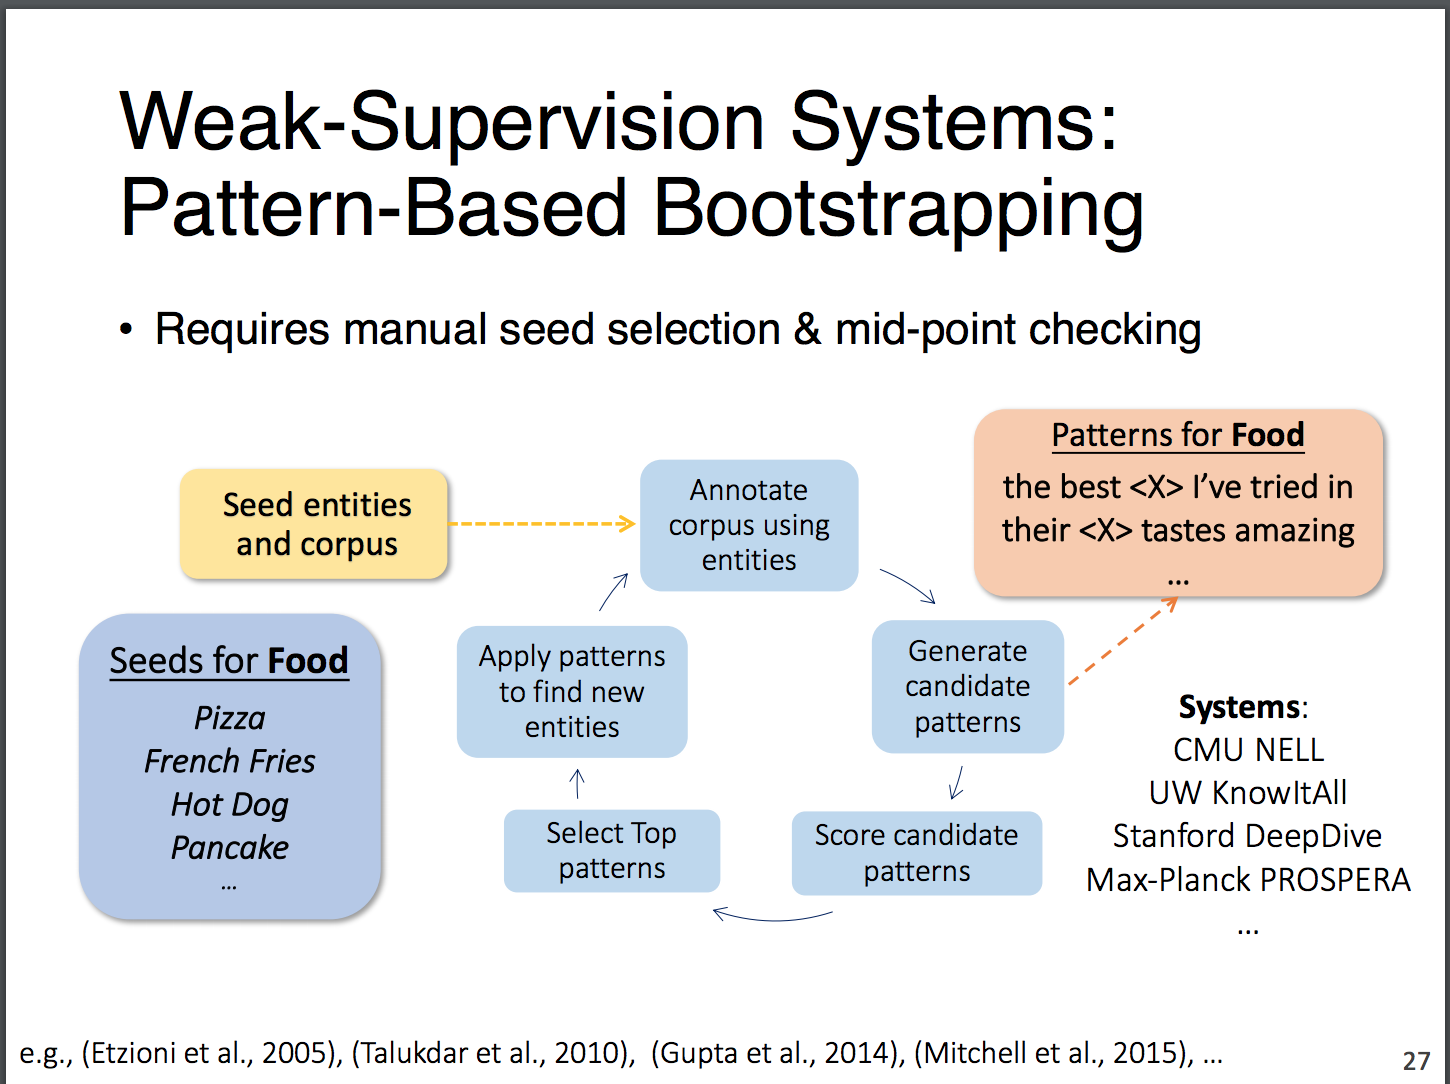
\includegraphics[scale=0.5]{fig0601/weak-supervision-ppt}
\end{figure}

\paragraph{Leveraging distance supervision.}
1. Detect entity names from text\\
2. Match name strings to KB entities.\\
3. Propagate types to the un-matchable names

LImitations:
\begin{itemize}
	\item Context-agnostic type prediction.
	\item Sparsity of contextual bridges (people describing the same things using different terms). This results in inefficient type propagation. 
\end{itemize}
Example: ClusType approach (KDD '15): type propagation + relation phrase clustering at the same time.\\
Smoothness assumption: if two nodes are similar saccording to the graph, then their type labels should also be similar.  

Two relation phrases should be grouped together if: (1) similar string; (2) similar context; (3) similar types for entity arguments. --> Multi-view clustering.

From coarse-grained typing to fine-grained entity typing:
For a clean mention, its "positive types" should be ranked higher than all its "negative types". 

Hierarchical type inference (Ren et al EMNLP '16)

Partial label embedding (PLE, KDD '16)\\

Comparison: WSABIE (Google ACL '15)
Predictive Text Embedding (MSR)

\paragraph{Prior works}
e.g: CoType approach (WWW '17)
Co-embedding for typing entities and relations

\subsubsection{Part 2: Joint extraction of typed entities and relations}
How to leverage other knowledge, such as the distributional statistics of characters and words, and annotations for other tasks and other domains, and the linguistics and problem structures, to combat the problem of inadequate supervision and conduct low-resource information extraction.

\paragraph{Traditional NER method} sequence tagging models, hand-engineering features

\paragraph{Neural NER models} e.g: RNN for representation. 

\paragraph{Distributional similarity of words}
Why not perform joint learning of word embeddings and NER?
\begin{figure}[h]
	\centering
	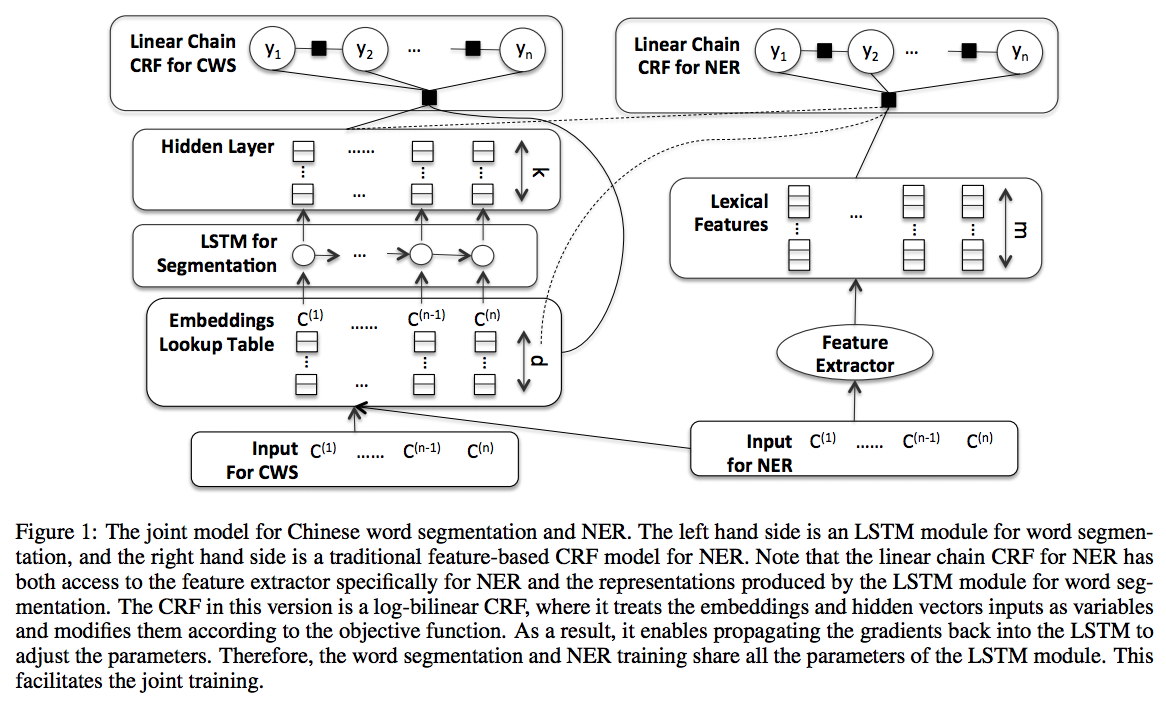
\includegraphics[scale=0.8]{fig0601/peng2015NER}
\end{figure}

e.g: chinese word boundaries

\paragraph{Sharing high-level representations} (Peng and Dredze, 2016)
\begin{figure}[h]
	\centering
	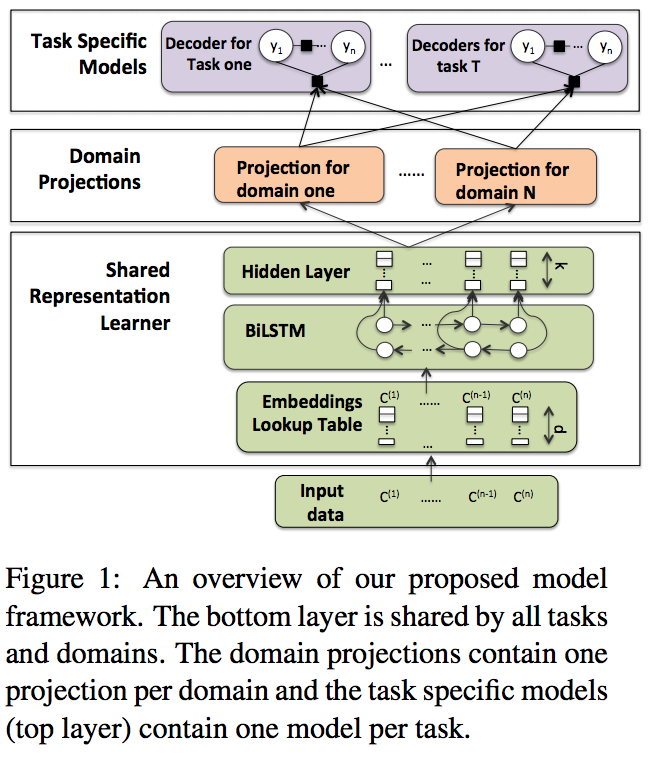
\includegraphics[scale=0.6]{fig0601/peng2016multi-task}
\end{figure}

\paragraph{Domains for languages}
Multi-task multi-domain learning. (Peng and Dredze, 2017) \\
Task-specific models  -- domain projections -- shared representation learner

\paragraph{How to build NER for a new language} using (1) comparable corpora (e.g. wikipedia) and (2) English NER tagger? (Want, Peng and Duh, 2017) \\
Motivation: learn a bilingual word embedding\\

Two approaches:
\begin{itemize}
	\item Fixed embeddings
	\item multi-task training
\end{itemize}

\paragraph{Encoding linguistic structures to improve}
e.g: cross-language N-ary relation extractions. Problem: hard to define the shortest path. Also, we are not allowed to go across the boundaries.
(Peng et al, 2017) representation learning framework.

$\bullet$ Goal; want to construct a representation learner, that captures difference types of dependencies over an \emph{acyclic graph}.

$\bullet$ Previous approaches: graph neural network, tree neural network, etc.
Problem: RNNs are expensive, and that information does not propagate to distant nodes.

$\bullet$ (Peng et al, 2017) cross-sentence n-ary relation extraction with graph LSTMs (in comparison to chain LSTM, there is one more forget gate per dependency)

$\bullet$ Multi-task learning from the shared representation learning


\subsection{Part 3: Recent advances in knowledge base reasoning}

\paragraph{Motivations} Knowledge Graphs are not complete. Missing links, etc.\\

$\bullet$ Knowledge graph supports various applications: structured search, QA, ASR, relation extraction, summarization, etc.

$\bullet$ Goal: complete the knowledge graph automatically (leveraging existing knowledge graph).

\paragraph{Path-based reasoning}
Why do we need path-based algorithms? (but not neural network embeddings) Explainability!
\begin{itemize}
	\item Path-ranking algorithm (Lao et al 2011) First random walk with restarts, then do LogReg to rank different paths (make paths leading to the correct destinations have higher weights)
	
	\item ProPPR, Wang et al 2013 PhD thesis and Want et al 2015. Generalizes PRA with recursive probabilistic logic programs. May use other relations to jointly infer this target relation.
	
	\item Subgraph feature extraction, Gardner et al 2015
	
	\item Chains of reasoning. Das et al 2017. PRA to derive path, then use RNNs to perform reasoning of the target relation.
	
\end{itemize}


\paragraph{Embedding-based reasoning}
Related method. (Robust and scalable)
\begin{itemize}
	\item RESCAL, Nickel et al, 2011. Tensor-based factorization. Head entity - tail entity - relation tensor. $Y=EWE^T$
	\item TransE, Bordes et al, 2013. If you have the initial embedding, and you add the relation to the head entity, you should get close to the target tail entity.
	\item Neural Tensor Network, Socher et al, 2013
	\item TransR / CTransR Lin et al 2015
	\item Complex Embeddings, Trouillon et al, 2016
	\item Poincar{\'e} embedding. Get out of the Euclidean space. Learn hierarchical KB representations by looking at hyperbolic space. $$d(u,v) = arcosh(1+2\frac{||u-v||^2}{(1-||u||^2)(1-||v||^2)})$$
	\item ConvE (Detters et al, AAAI 2018) learn entities with CNN. Reshape head and relation embeddings into "images".
\end{itemize}


\paragraph{Bridging path-based and embedding-based reasoning}: DeepPath, MINERVA, and DIVA\\
\begin{itemize}
	\item RL for KB reasoning: DeepPath (Xiong et al 2017 EMNLP). Path finding as a MDP. Train RL agent to find paths. Represent KG with pretrained KG embeddings. Use he learned paths as logical formulas.
	\item MINERVA: Das et al ICLR 2018. Go for a walk and arrive at the answer.
	\item DIVA: Variational KB reasoning. Inferring latent paths connecting entity nodes.
\end{itemize}

Sidenote: RL is a general purpose framework for decision making. 



\subsection{T5: Socially Responsible NLP}
\paragraph{Speakers} Professors Yulia Tsvetkov, Vinodkumar Prabhakaran, Rob Voigt \\
(ref: CMU CS11830)

$\bullet$ Be careful: nobody is expert simultaneously in all of the sociology + psychology + linguistic + CSC + ML + statistics. 

\subsubsection{Ethics in NLP: foundations}

$\bullet$ What is ethics? About doing the good / right things. Problem: sometimes cannot define good / bad properly. 

$\bullet$ Another example: the chicken classifier (hen -> egg farm; roster -> meat farm)

$\bullet$ Ethics versus law

$\bullet$ Identify a range of problems / questions we should ask when building NLP systems.

$\bullet$ E.g: the A.I. "Gaydar"

\subsubsection{Technical Aspects}
\paragraph{Humans are the "natural" in NLP}
In a way, NLP is human subjects research.

$\bullet$ Self-selection bias. e.g: who posts on Yelp

$\bullet$ Reporting bias. e.g: People do not necessarily talk about things in the world in proportion to their empirical distributions.

$\bullet$ (Jurgens et al ACL 17) Socioeconomic bias in language identification.

\subsubsection{Case study}

$\bullet$ The semantic of words contain inherent biases. e.g: the bias embedding test. Might be able to exclude some of them using fair learning. \\
/* Excluding gender differences from semantic embeddings is possible, but how about languages like French, where gender difference is encoded as syntactic rules? */


\subsubsection{Test}

$\bullet$ Should care about whether the task is beneficial to the people involved. The purpose is not going to build "gaydar" or "tell the race of driver based on the police officer's speeches". 

$\bullet$ There can be multiple causes for an effect. We should not give blatant judgements without fully assessing them. For example, among those pulled over \emph{only for minor ticketing}, African Americans receive more tickets for minor car damages. This could due to biases in police officers. This could also due to their economic status (less frequently go to repair the cars once damaged? ), etc.

$\bullet$ There are complicated reasons behind these problems. Be careful when organizing sentences, etc.

$\bullet$ Extension: CS294 fair learning. Also Graeme Hirst's CSC D03 (social impacts of ML).

\takeaway{People are focusing more on the fairness of machine learning. ML researches should take more social responsibilities: Present the researches in an explainable manner, and explore the indications of the researches.}
